\documentclass[a4paper,11pt]{article}

% Kodovani (cestiny) v dokumentu: utf-8
%\usepackage[cp1250]{inputenc}	% Omezena stredoevropska kodova stranka, pouze MSW.
\usepackage[utf8]{inputenc}	% Doporucujeme pouzivat UTF-8 (unicode).

\usepackage[margin=2cm]{geometry}
\newtoks\jmenopraktika \newtoks\jmeno \newtoks\datum
\newtoks\obor \newtoks\skupina \newtoks\rocnik \newtoks\semestr
\newtoks\cisloulohy \newtoks\jmenoulohy
\newtoks\tlak \newtoks\teplota \newtoks\vlhkost

\jmenopraktika={Fyzikální praktikum 1}
\jmeno={Lukáš Lejdar}
\datum={8. října 2024}
\obor={F}
\skupina={Út 16:00}

\cisloulohy={1}
\jmenoulohy={Odraz a lom světla, Fresnelovy vztahy, Snellův zákon}

\tlak={101{,}35}
\teplota={21,1}
\vlhkost={47,7}


%%%%%%%%%%% Uzitecne balicky:
\usepackage[czech]{babel}
\addto\captionsczech{\renewcommand{\figurename}{Obrázek}}

\usepackage{graphicx}
\usepackage{amsmath}
\usepackage{xspace}
\usepackage{url}
\usepackage{indentfirst}
\usepackage{wrapfig}
\usepackage{xcolor}
\usepackage{subfig}
\usepackage{subcaption}
\usepackage{enumitem}
\usepackage{tikzsymbols}
\usepackage{newfloat}

\DeclareFloatingEnvironment[fileext=lof]{graph}
\captionsetup[graph]{labelformat=simple, labelsep=colon, name=Graf}

%%%%%% Zamezeni parchantu:
\widowpenalty 10000 \clubpenalty 10000 \displaywidowpenalty 10000
%%%%%% Parametry pro moznost vsazeni vetsiho poctu obrazku na stranku
\setcounter{topnumber}{3}	  % max. pocet floatu nahore (specifikace t)
\setcounter{bottomnumber}{3}	  % max. pocet floatu dole (specifikace b)
\setcounter{totalnumber}{6}	  % max. pocet floatu na strance celkem
\renewcommand\topfraction{0.9}	  % max podil stranky pro floaty nahore
\renewcommand\bottomfraction{0.9} % max podil stranky pro floaty dole
\renewcommand\textfraction{0.1}	  % min podil stranky, ktery musi obsahovat text
\intextsep=8mm \textfloatsep=8mm  %\intextsep pro ulozeni [h] floatu a \textfloatsep pro [b] or [t]

% Tecky za cisly sekci:
\renewcommand{\thesection}{\arabic{section}.}
\renewcommand{\thesubsection}{\thesection\arabic{subsection}.}
% Jednopismenna mezera mezi cislem a nazvem kapitoly:
\makeatletter \def\@seccntformat#1{\csname the#1\endcsname\hspace{1ex}} \makeatother
%
\newcommand{\vsn}[4]{\ensuremath{#1 =} #2(#3)\,#4}
\newcommand{\vrn}[6]{\ensuremath{#1 =} (#2 $\pm$ #3)\,#4 ($p=$ #5\,\%, $\nu=$ #6)}

\newcommand*\circled[1]{\tikz[baseline=(char.base)]{
		\node[shape=circle,draw,inner sep=1pt] (char) {#1};}}

%%%%%%%%%%%%%%%%%%%%%%%%%%%%%%%%%%%%%%%%%%%%%%%%%%%%%%%%%%%%%%%%%%%%%%%%%%%%%%%
% Zacatek dokumentu
%%%%%%%%%%%%%%%%%%%%%%%%%%%%%%%%%%%%%%%%%%%%%%%%%%%%%%%%%%%%%%%%%%%%%%%%%%%%%%%

\begin{document}

\thispagestyle{empty}

{
\begin{center}
\sf 
{\Large Ústav fyziky a technologií plazmatu Přírodovědecké fakulty Masarykovy univerzity} \\
\bigskip
{\huge \bfseries FYZIKÁLNÍ PRAKTIKUM} \\
\bigskip
{\Large \the\jmenopraktika}
\end{center}

\bigskip

\sf
\noindent
\setlength{\arrayrulewidth}{1pt}
\begin{tabular*}{\textwidth}{@{\extracolsep{\fill}} l l}
\large {\bfseries Zpracoval:}  \the\jmeno & \large  {\bfseries Naměřeno:} \the\datum\\[2mm]
\large  {\bfseries Obor:} \the\obor  \hspace{40mm}  {\bfseries Skupina:} \the\skupina %
&\large {\bfseries Testováno:}\\
\\
\hline
\end{tabular*}
}

\bigskip

{
\sf
\noindent \begin{tabular}{p{4cm} p{0.6\textwidth}}
\Large  Úloha č. {\bfseries \the\cisloulohy:} \par
\smallskip
$T=\the\teplota$~$^\circ$C \par
$p=\the\tlak$~kPa \par
$\varphi=\the\vlhkost$~\%
&\Large \bfseries \the\jmenoulohy  \\[2mm]
\end{tabular}
}


\section{Úvod}

V úloze budu měřit odrazivost s a p polarizovaného světla na dielektriku v závislosti na úhlu dopadu. Odtud určím Brewsterův úhel a několika metodami dopočítám index lomu. V druhé části budu měřit index lomu planparalelní desky z posuvu paprsku.
 
\section{Postup měření}

\subsection{Měření odrazivosti dielektrika}

Měření bude probíhat podle uspořádání na obrázku 1. Lineárně polarizovaný laser dopadá na vzorek, odkud se odráží na detektor, který měří buzené napětí $ U_R $ úměrné jeho intenzitě $ I_R $. Intenzitu před odrazem $ I_0 \propto U_0  $ zjistím na začátku, kdy vzorek odejmu a detektor umístím do polohy A.

Pro polarizace $ p $ a $ s $ změřím závislost napětí na úhlu dopadu a získané hodnoty přepočítám na odrazivost podle $ R = \frac{I_R}{I_0} = \frac{U_R}{U_0} $. Pro odrazivost $ R_p $ bych měl najít tzv. Brewsterův úhel $ \varphi_B  $, pro který platí $ R_p(\varphi_B) = 0 $. V jeho okolí potom měření zopakuji s použitím zesíleného signálu a jeho hodnotu zpřesním. Podle Brewsterova zákona potom platí $  $

\begin{equation}
\tan \varphi_B = n,
\end{equation}


\noindent
kde n je index lomu. Tuto hodnotu zároveň můžu spočítat ze Snellova zákona a Fresnelových vztahů buď fitem, nebo vyjádřením $ n $.

\begin{equation}
n_0 \sin\varphi_0 = n \sin\varphi_1
\end{equation}

\begin{align}
    \sqrt{R_p} = \frac{n_0 \cos(\varphi_1) - n \cos(\varphi_0)}{n_0 \cos(\varphi_1) + n \cos(\varphi_0)} \qquad
\sqrt{R_s}  = \frac{n_0 \cos(\varphi_0) - n \cos(\varphi_1)}{n_0 \cos(\varphi_0) + n \cos(\varphi_1)}
\end{align}

\begin{flalign}
   &\text{\textbf{\circled{1}} } \varphi_0 < \varphi_B & n = \sqrt{\frac{(1 + \sqrt{R_s})(1 + \sqrt{R_p} )}{ (1 - \sqrt{R_s} )(1 - \sqrt{R_p} ) }}  && \\[10pt]
   &\text{\textbf{\circled{2}} } \varphi_0 > \varphi_B & n = \sqrt{\frac{(1 + \sqrt{R_s})(1 - \sqrt{R_p} )}{ (1 - \sqrt{R_s} )(1 + \sqrt{R_p} ) }}  &&
\end{flalign}

\newpage

\begin{figure}[htpb]
    \centering
    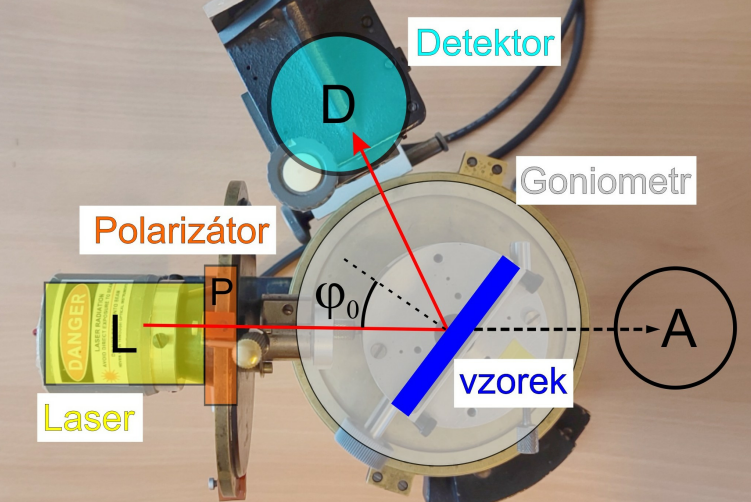
\includegraphics[width=0.4\textwidth]{odraz_aparatura.png}
    \caption{Experimentální uspořádání pro měření úhlové závislosti odrazivosti dielektrika. Poloha detektoru A odpovídá referenční pozici pro měření signálu bez vzorku}
\end{figure}

\subsection{Průchod světla planparalelní deskou}

Obrázek 2 zobrazuǰe průchod světla planparalelní deskou a obrázek 3 realizaci tohoto jevu. Svazek světla dopadá na vzorek pod úhlem $ \alpha $, který ho tím translačně posouvá o vzdálenost $ x $. Ze Snellova zákona potom vyplývá vztah pro výpočet indexu lomu vzorku 


\begin{align}
n = n_0 \sqrt{\sin^2 \alpha + (1 - \frac{x}{d \sin \alpha})^{-2} \cos^2 \alpha } \\ \notag
\end{align}


Změřím velikost odchylky $ x $ pro několik úhlů $ \alpha $ a výsledné hodnoty zprůměruju.

\begin{figure}[htpb]
    \centering
    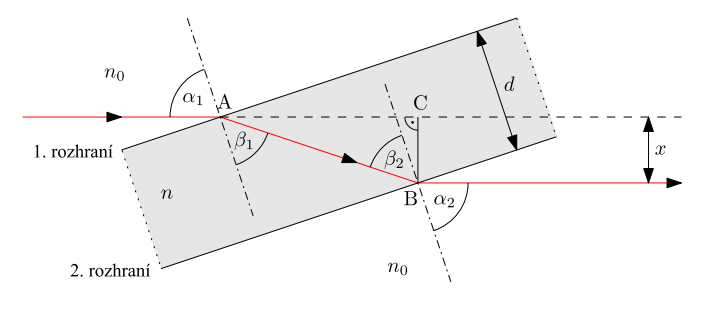
\includegraphics[width=0.6\textwidth]{planparalelni_deska.png}
    \caption{Průchod světla planparalelní deskou}
\end{figure}

\begin{figure}[htpb]
    \centering
    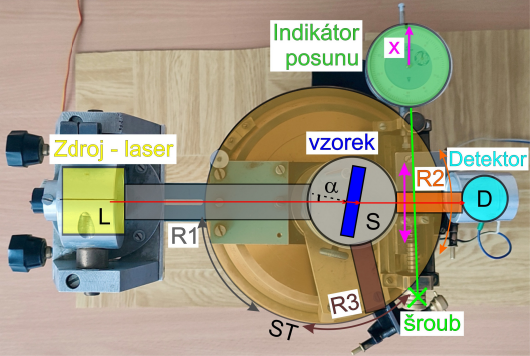
\includegraphics[width=0.4\textwidth]{planparalela_aparatura.png}
    \caption{Experimentální uspořádání pro měření průchodu světla planparalelní deskou a hranolem}
\end{figure}

\section{Výsledky měření}

\subsection{Měření odrazivosti dielektrika}

Sestavil jsem měření podle obrázku 1 a měřil intenzitu světla dopadajícího na detektor v rozmezí úhlu dopadu $ [25, 85]^{\circ} $ pro obě polarizace. Použité dielektrikum bylo v tomto případě sklo. Hodnoty převedené na odrazivost jsou v grafu 1, odkud je vidět, že Brewsterův úhel je někde kolem 55$ ^{\circ} $. V~okolí tohoto úhlu jsem měřil znovu při zesílení signálu, výsledky vynesl do grafu 2 a odečetl přesnější hodnotu $ \varphi_B = 56 ^{\circ} $. Výsledný index lomu spočítám několika způsoby :

\begin{table}[htpb]
    \centering
    \begin{tabular}{ll}
    \hline \hline
    metoda & n \\ \hline
    výpočet podle vztahu (1) & 1.48 \\
    výpočet podle vztahů (4) a (5) & $1.45 \pm 0.02$ \\
    fit odrazivostí v s polarizaci & $1.45 \pm 0.01$ \\
    fit odrazivostí v p polarizaci & $1.49 \pm 0.03$ \\
    \hline \hline
    \end{tabular}
    \caption{výsledné indexy lomu vzorku}
\end{table}

\vspace{-30pt}

\begin{table}[htpb]
    \begin{minipage}[b]{.54\linewidth}
        \centering
        \resizebox{\textwidth}{!}{ % GNUPLOT: LaTeX picture with Postscript
\begingroup
  \makeatletter
  \providecommand\color[2][]{%
    \GenericError{(gnuplot) \space\space\space\@spaces}{%
      Package color not loaded in conjunction with
      terminal option `colourtext'%
    }{See the gnuplot documentation for explanation.%
    }{Either use 'blacktext' in gnuplot or load the package
      color.sty in LaTeX.}%
    \renewcommand\color[2][]{}%
  }%
  \providecommand\includegraphics[2][]{%
    \GenericError{(gnuplot) \space\space\space\@spaces}{%
      Package graphicx or graphics not loaded%
    }{See the gnuplot documentation for explanation.%
    }{The gnuplot epslatex terminal needs graphicx.sty or graphics.sty.}%
    \renewcommand\includegraphics[2][]{}%
  }%
  \providecommand\rotatebox[2]{#2}%
  \@ifundefined{ifGPcolor}{%
    \newif\ifGPcolor
    \GPcolorfalse
  }{}%
  \@ifundefined{ifGPblacktext}{%
    \newif\ifGPblacktext
    \GPblacktexttrue
  }{}%
  % define a \g@addto@macro without @ in the name:
  \let\gplgaddtomacro\g@addto@macro
  % define empty templates for all commands taking text:
  \gdef\gplbacktext{}%
  \gdef\gplfronttext{}%
  \makeatother
  \ifGPblacktext
    % no textcolor at all
    \def\colorrgb#1{}%
    \def\colorgray#1{}%
  \else
    % gray or color?
    \ifGPcolor
      \def\colorrgb#1{\color[rgb]{#1}}%
      \def\colorgray#1{\color[gray]{#1}}%
      \expandafter\def\csname LTw\endcsname{\color{white}}%
      \expandafter\def\csname LTb\endcsname{\color{black}}%
      \expandafter\def\csname LTa\endcsname{\color{black}}%
      \expandafter\def\csname LT0\endcsname{\color[rgb]{1,0,0}}%
      \expandafter\def\csname LT1\endcsname{\color[rgb]{0,1,0}}%
      \expandafter\def\csname LT2\endcsname{\color[rgb]{0,0,1}}%
      \expandafter\def\csname LT3\endcsname{\color[rgb]{1,0,1}}%
      \expandafter\def\csname LT4\endcsname{\color[rgb]{0,1,1}}%
      \expandafter\def\csname LT5\endcsname{\color[rgb]{1,1,0}}%
      \expandafter\def\csname LT6\endcsname{\color[rgb]{0,0,0}}%
      \expandafter\def\csname LT7\endcsname{\color[rgb]{1,0.3,0}}%
      \expandafter\def\csname LT8\endcsname{\color[rgb]{0.5,0.5,0.5}}%
    \else
      % gray
      \def\colorrgb#1{\color{black}}%
      \def\colorgray#1{\color[gray]{#1}}%
      \expandafter\def\csname LTw\endcsname{\color{white}}%
      \expandafter\def\csname LTb\endcsname{\color{black}}%
      \expandafter\def\csname LTa\endcsname{\color{black}}%
      \expandafter\def\csname LT0\endcsname{\color{black}}%
      \expandafter\def\csname LT1\endcsname{\color{black}}%
      \expandafter\def\csname LT2\endcsname{\color{black}}%
      \expandafter\def\csname LT3\endcsname{\color{black}}%
      \expandafter\def\csname LT4\endcsname{\color{black}}%
      \expandafter\def\csname LT5\endcsname{\color{black}}%
      \expandafter\def\csname LT6\endcsname{\color{black}}%
      \expandafter\def\csname LT7\endcsname{\color{black}}%
      \expandafter\def\csname LT8\endcsname{\color{black}}%
    \fi
  \fi
    \setlength{\unitlength}{0.0500bp}%
    \ifx\gptboxheight\undefined%
      \newlength{\gptboxheight}%
      \newlength{\gptboxwidth}%
      \newsavebox{\gptboxtext}%
    \fi%
    \setlength{\fboxrule}{0.5pt}%
    \setlength{\fboxsep}{1pt}%
    \definecolor{tbcol}{rgb}{1,1,1}%
\begin{picture}(5328.00,3600.00)%
    \gplgaddtomacro\gplbacktext{%
      \csname LTb\endcsname%%
      \put(134,720){\makebox(0,0)[r]{\strut{}$0$}}%
      \put(134,1020){\makebox(0,0)[r]{\strut{}$0.1$}}%
      \put(134,1320){\makebox(0,0)[r]{\strut{}$0.2$}}%
      \put(134,1620){\makebox(0,0)[r]{\strut{}$0.3$}}%
      \put(134,1920){\makebox(0,0)[r]{\strut{}$0.4$}}%
      \put(134,2219){\makebox(0,0)[r]{\strut{}$0.5$}}%
      \put(134,2519){\makebox(0,0)[r]{\strut{}$0.6$}}%
      \put(134,2819){\makebox(0,0)[r]{\strut{}$0.7$}}%
      \put(134,3119){\makebox(0,0)[r]{\strut{}$0.8$}}%
      \put(134,3419){\makebox(0,0)[r]{\strut{}$0.9$}}%
      \put(266,500){\makebox(0,0){\strut{}$20$}}%
      \put(951,500){\makebox(0,0){\strut{}$30$}}%
      \put(1636,500){\makebox(0,0){\strut{}$40$}}%
      \put(2321,500){\makebox(0,0){\strut{}$50$}}%
      \put(3005,500){\makebox(0,0){\strut{}$60$}}%
      \put(3690,500){\makebox(0,0){\strut{}$70$}}%
      \put(4375,500){\makebox(0,0){\strut{}$80$}}%
      \put(5060,500){\makebox(0,0){\strut{}$90$}}%
    }%
    \gplgaddtomacro\gplfronttext{%
      \csname LTb\endcsname%%
      \put(1586,3246){\makebox(0,0)[r]{\strut{}fit $R_p(\varphi)$}}%
      \csname LTb\endcsname%%
      \put(1586,3026){\makebox(0,0)[r]{\strut{}fit $R_s(\varphi)$}}%
      \csname LTb\endcsname%%
      \put(-471,2069){\rotatebox{-270.00}{\makebox(0,0){\strut{}odrazivost}}}%
      \put(2663,170){\makebox(0,0){\strut{}úhel dopadu $\varphi$ (°)}}%
    }%
    \gplbacktext
    \put(0,0){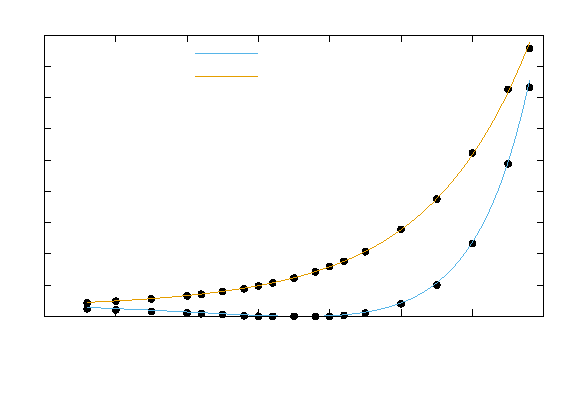
\includegraphics[width={266.40bp},height={180.00bp}]{odrazivost}}%
    \gplfronttext
  \end{picture}%
\endgroup
 }
        \captionsetup{type=graph}
        \caption{Závislost odrazivosti $ R_p $ a $ R_s $ na úhlu dopadu}
    \end{minipage} 
    \hfill
    \begin{minipage}[b]{.42\linewidth}
        \centering
        \resizebox{\textwidth}{!}{ % GNUPLOT: LaTeX picture with Postscript
\begingroup
  \makeatletter
  \providecommand\color[2][]{%
    \GenericError{(gnuplot) \space\space\space\@spaces}{%
      Package color not loaded in conjunction with
      terminal option `colourtext'%
    }{See the gnuplot documentation for explanation.%
    }{Either use 'blacktext' in gnuplot or load the package
      color.sty in LaTeX.}%
    \renewcommand\color[2][]{}%
  }%
  \providecommand\includegraphics[2][]{%
    \GenericError{(gnuplot) \space\space\space\@spaces}{%
      Package graphicx or graphics not loaded%
    }{See the gnuplot documentation for explanation.%
    }{The gnuplot epslatex terminal needs graphicx.sty or graphics.sty.}%
    \renewcommand\includegraphics[2][]{}%
  }%
  \providecommand\rotatebox[2]{#2}%
  \@ifundefined{ifGPcolor}{%
    \newif\ifGPcolor
    \GPcolorfalse
  }{}%
  \@ifundefined{ifGPblacktext}{%
    \newif\ifGPblacktext
    \GPblacktexttrue
  }{}%
  % define a \g@addto@macro without @ in the name:
  \let\gplgaddtomacro\g@addto@macro
  % define empty templates for all commands taking text:
  \gdef\gplbacktext{}%
  \gdef\gplfronttext{}%
  \makeatother
  \ifGPblacktext
    % no textcolor at all
    \def\colorrgb#1{}%
    \def\colorgray#1{}%
  \else
    % gray or color?
    \ifGPcolor
      \def\colorrgb#1{\color[rgb]{#1}}%
      \def\colorgray#1{\color[gray]{#1}}%
      \expandafter\def\csname LTw\endcsname{\color{white}}%
      \expandafter\def\csname LTb\endcsname{\color{black}}%
      \expandafter\def\csname LTa\endcsname{\color{black}}%
      \expandafter\def\csname LT0\endcsname{\color[rgb]{1,0,0}}%
      \expandafter\def\csname LT1\endcsname{\color[rgb]{0,1,0}}%
      \expandafter\def\csname LT2\endcsname{\color[rgb]{0,0,1}}%
      \expandafter\def\csname LT3\endcsname{\color[rgb]{1,0,1}}%
      \expandafter\def\csname LT4\endcsname{\color[rgb]{0,1,1}}%
      \expandafter\def\csname LT5\endcsname{\color[rgb]{1,1,0}}%
      \expandafter\def\csname LT6\endcsname{\color[rgb]{0,0,0}}%
      \expandafter\def\csname LT7\endcsname{\color[rgb]{1,0.3,0}}%
      \expandafter\def\csname LT8\endcsname{\color[rgb]{0.5,0.5,0.5}}%
    \else
      % gray
      \def\colorrgb#1{\color{black}}%
      \def\colorgray#1{\color[gray]{#1}}%
      \expandafter\def\csname LTw\endcsname{\color{white}}%
      \expandafter\def\csname LTb\endcsname{\color{black}}%
      \expandafter\def\csname LTa\endcsname{\color{black}}%
      \expandafter\def\csname LT0\endcsname{\color{black}}%
      \expandafter\def\csname LT1\endcsname{\color{black}}%
      \expandafter\def\csname LT2\endcsname{\color{black}}%
      \expandafter\def\csname LT3\endcsname{\color{black}}%
      \expandafter\def\csname LT4\endcsname{\color{black}}%
      \expandafter\def\csname LT5\endcsname{\color{black}}%
      \expandafter\def\csname LT6\endcsname{\color{black}}%
      \expandafter\def\csname LT7\endcsname{\color{black}}%
      \expandafter\def\csname LT8\endcsname{\color{black}}%
    \fi
  \fi
    \setlength{\unitlength}{0.0500bp}%
    \ifx\gptboxheight\undefined%
      \newlength{\gptboxheight}%
      \newlength{\gptboxwidth}%
      \newsavebox{\gptboxtext}%
    \fi%
    \setlength{\fboxrule}{0.5pt}%
    \setlength{\fboxsep}{1pt}%
    \definecolor{tbcol}{rgb}{1,1,1}%
\begin{picture}(4320.00,3744.00)%
    \gplgaddtomacro\gplbacktext{%
      \csname LTb\endcsname%%
      \put(84,748){\makebox(0,0)[r]{\strut{}$0$}}%
      \put(84,1149){\makebox(0,0)[r]{\strut{}$0.1$}}%
      \put(84,1550){\makebox(0,0)[r]{\strut{}$0.2$}}%
      \put(84,1951){\makebox(0,0)[r]{\strut{}$0.3$}}%
      \put(84,2352){\makebox(0,0)[r]{\strut{}$0.4$}}%
      \put(84,2753){\makebox(0,0)[r]{\strut{}$0.5$}}%
      \put(84,3154){\makebox(0,0)[r]{\strut{}$0.6$}}%
      \put(84,3555){\makebox(0,0)[r]{\strut{}$0.7$}}%
      \put(216,528){\makebox(0,0){\strut{}$50$}}%
      \put(702,528){\makebox(0,0){\strut{}$51$}}%
      \put(1188,528){\makebox(0,0){\strut{}$52$}}%
      \put(1674,528){\makebox(0,0){\strut{}$53$}}%
      \put(2160,528){\makebox(0,0){\strut{}$54$}}%
      \put(2645,528){\makebox(0,0){\strut{}$55$}}%
      \put(3131,528){\makebox(0,0){\strut{}$56$}}%
      \put(3617,528){\makebox(0,0){\strut{}$57$}}%
      \put(4103,528){\makebox(0,0){\strut{}$58$}}%
      \put(2766,1237){\makebox(0,0)[l]{\strut{}$(\varphi_B, 0.032)$}}%
    }%
    \gplgaddtomacro\gplfronttext{%
      \csname LTb\endcsname%%
      \put(-521,2151){\rotatebox{-270.00}{\makebox(0,0){\strut{}U (mV)}}}%
      \put(2159,198){\makebox(0,0){\strut{}úhel dopadu $\varphi$ (°)}}%
    }%
    \gplbacktext
    \put(0,0){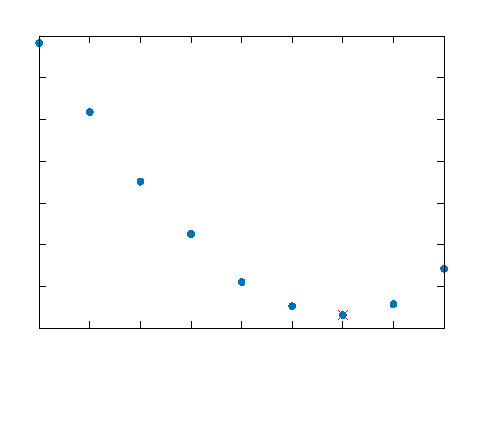
\includegraphics[width={216.00bp},height={187.20bp}]{brewster_uhel}}%
    \gplfronttext
  \end{picture}%
\endgroup
 } \\
    \captionsetup{type=graph}
    \caption{Měření $ R_p $ odrazivosti v okolí $ \varphi_B $}
    \end{minipage} 
\end{table}

\subsection{Průchod světla planparalelní deskou}

\begin{wrapfigure}[13]{tr}{0.44\textwidth}
    \vspace{-25pt}
    \centering
    \begin{tabular}{l l l}
        \hline\hline
        $ \varphi (^{\circ}) $ & $ x $ (mm) & n \\
        \hline
        5  & 0.27 & 1.440 \\
        10 & 0.61 & 1.520 \\
        15 & 0.97 & 1.557 \\
        20 & 1.20 & 1.480 \\
        25 & 1.56 & 1.490 \\
        30 & 1.94 & 1.492 \\
        35 & 2.36 & 1.497 \\
        40 & 2.77 & 1.483 \\
        45 & 3.21 & 1.466 \\
        50 & 3.77 & 1.469 \\
        \hline\hline
    \end{tabular}
    \captionsetup{type=table}
    \caption{měření indexu lomu z úhlu dopadu $ \alpha $ a odchylky x}
\end{wrapfigure}

Jako vzorek jsem použil sklo ze stejného materiálu jako v první části úlohy a vložil ho do aparatury z obrázku 3. Postupně jsem měnil natočení vzorku vůči laseru o úhly $ \alpha $ v rozmezí $ [5^{\circ}:50^{\circ}] $ a odečítal odchylku od původní trajektorie. Výsledné hodnoty jsou uvedené v tabulce 2 s výpočtem indexu lomu pro každé měření podle vztahu (6). Ze statistického rozboru jsem určil finální hodnotu

\begin{equation*}
n = 1.49 \pm 0.04
\end{equation*}

\newpage

\section{Závěr}

Změřil jsem závislost odrazivosti s a p polarizovaného světla při dopadu na skleněný vzorek a výsledné hodnoty vynesl do grafu 1. Fit je podle teoretických vztahů (2) a (3), odkud jsem určil index lomu vzorku prvním způsobem. Odrazivost $ R_p $ bylo potom potřeba znovu zjistit citlivěji v okolí, kde $ R_p \approx 0 $ pro přesnější určení Brewsterova úhlu $ \varphi_B = 56 ^{\circ}   $. Index lomu je pak dál dopočítaný i podle vztahů~(1),~nebo (4) a (5). Všechny čtyři výsledné hodnoty jsou uvedené v tabulce 1. 

V druhé části úlohy jsem použil planparalelní desku ze stejného materiálu jako v první čási a měřil index lomu z posunutí paprsku světla po průchodu vzorkem natočeným vůči paprsku o nějaký úhel. 

Ve výsledných hodnotách ze všech metod existuje trend podle kterého je $ n \approx 1.49 $ a druhý, který říká, že $ n \approx 1.45 $. Přikláněl bych se spíš hodnotě $ 1.49 $, protože vychází z více nezávislých měření. Na druhé straně do čísla $ 1.45 $ se v obou případech nějakým způsobem míchalo měření $ R_s $, které tím můžeme podezírat z nějaké chyby.


\end{document}
